\documentclass[12pt,a4paper]{report}
\usepackage[utf8]{inputenc}
\usepackage[pdftex]{graphicx}
\title{Pflichtenheft\\Beat The Score\\ 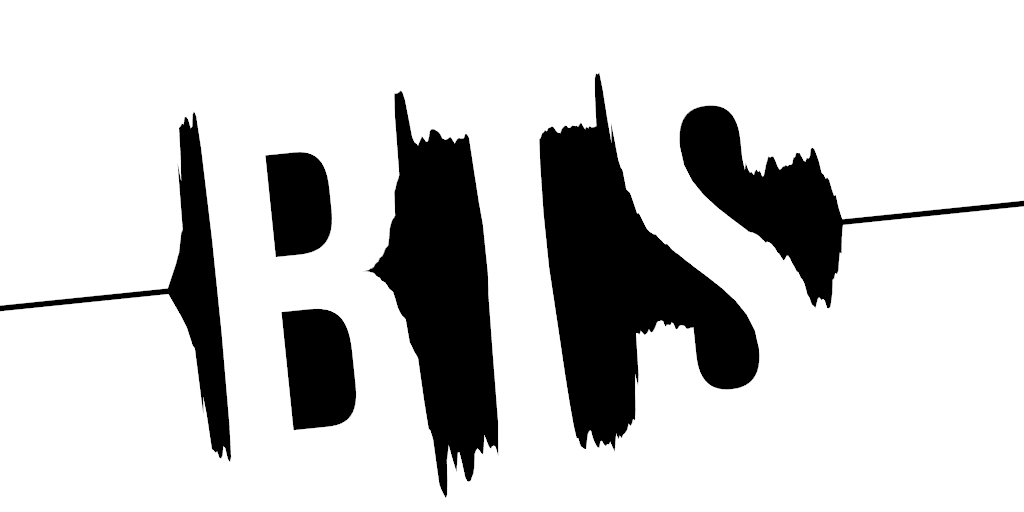
\includegraphics[scale=0.25]{Logo.png}}
\author{Felix Kugler \and Alfred Neumayer \and Daniel Novotny}
\date{12. Dezember 2013}

\renewcommand{\contentsname}{Inhalt}
\renewcommand{\chaptername}{Teil}
\begin{document}
  \maketitle
  \tableofcontents
  \chapter{Zielbestimmung}
    \section{Projektziele und Motivation}
      Ungeübte Musiker haben oft das Problem, dass es ihnen schwer fällt, Fehler zu erkennen. Daher soll eine App entwickelt werden, die den Benutzer durch visuelles Feedback in Echtzeit auf solche Fehler hinweist.
    \section{Umfang des Projekts}
    		\subsection{Kurzbeschreibung}
      Das Projekt umfasst die Entwicklung einer App zum Üben von Musikstücken, welche den Benutzer visuell auf Fehler hinweist und die Leistung des Benutzers bewertet. Das Musik-Instrument muss dazu an den Computer angeschlossen werden.\\
      
      	\subsection{Detailbeschreibung}
      		\subsubsection{Projektarbeit}
      Die Projektarbeit beschränkt sich auf die Unterstützung von MIDI-Geräten mit Schwerpunkt auf Klavier.
      Die App wird für Windows, Linux und Android entwickelt.
      Teil des Projektes ist die Implementierung des grundlegenden Spielablaufs auf Windows. \\
      In der Projektarbeit wird die Implementierung der Behandlung von MIDI-Signalen durchgeführt, der Schwerpunkt liegt dabei bei der Verwendung von Tasteninstrumenten. Die Projektarbeit beinhaltet weiterhin die Portierung auf Linux und Android. \\
      Dies ergibt folgende Anforderungen für die Projektarbeit: \\
      		\begin{itemize}
      		\item Ein Menü-System zur Navigation innerhalb des Programms, Auswahl von Spielmodi und Selektion von Optionen
      		\item Parser für das GP5-Dateiformat
      		\item Behandlung von Eingabesignalen verbundener MIDI-Geräte
      		\item Implementierung eines Synthesizers zur Audio-Ausgabe von Instrumenten-Geräuschen
			\item Audio-Ausgabe von gespielten Noten sowie Noten von Begleitspuren   
			\item Erkennung der Genauigkeit der Eingabe des Benutzers
			\item Anzeige der Genauigkeit während des Spiels
			\item Funktionsfähiges Programm für Windows, Linux und Android
			\end{itemize}
      		\subsubsection{Diplomarbeit}
      		Durch die Diplomarbeit soll die Projektarbeit um weitere funktionale Erweiterungen verbessert werden.
      		Die Reduzierung auf Klaviere wird aufgehoben und die verwendbaren Instrumente werden um Saiteninstrumente erweitert.
      		Der Schwerpunkt der Diplomarbeit bezieht sich auf die Erkennung und die Genauigkeitsüberprüfung von analogen Audiosignalen und Erweiterung des Spielkonzepts durch Behandlung von Bendings und Legato-Techniken.
      		Zusätzlich zum entstehenden Spiel wird die Implementierung einer Vertriebsplatform durchgeführt, um die Verkaufsabwicklung (geschieht über PayPal) zu ermöglichen und Aktualisierungen der Anwendung auf den Desktop-Systemen Windows und Linux zur Verfügung zu stellen.
      		Der Erfolg der Diplomarbeit wird somit durch folgenden Anforderungen definiert:
      		\begin{itemize}
      			\item Erweiterung der Eingabemöglichkeiten durch Erkennung und Behandlung analoger Audiosignale
      			\item Erkennung und Behandlung komplexer Legato-Techniken und Bendings bei der Eingabe
      			\item Ansprechende und Ergonomische Präsentation der zu spielenden Noten und der Korrekturen
      			\item Implementierung einer Vertriebs-Webseite für den Kauf des Spiels über PayPal
      			\item Behandlung der automatisierten Verkaufsabwicklung
      			\item Aufbau und Verwendung eines automatisierten Update-Systems
      		\end{itemize}
    \section{Performance und Ressourcen}
      Während Ladezeiten im Hauptmenü möglich sind, muss die Antwortzeit während dem Spielen unter 10 Millisekunden gehalten werden, da größere Latenzen deutlich hörbar sind.
      \subsection{Hardwarevoraussetzung}
      \begin{description}
      \item Windows und Linux:
      	\begin{itemize}
      	\item Festplattenspeicher: maximal 500 Megabyte
      	\item Arbeitsspeicher: maximal 1 Gigabyte
      	\item Prozessor: mindestens 2 GHz Dual-Core x86 Prozessor
      	\end{itemize}
      \item Android:
      	\begin{itemize}
      	\item Festplattenspeicher: maximal 250 Megabyte
      	\item Arbeitsspeicher: maximal 500 Megabyte
      	\item Prozessor: mindestens 1 GHz Dual-Core ARMv7 Prozessor
      	\end{itemize}
      \end{description}
    \section{Mengengerüste}
      \begin{itemize}
        \item Anzahl Lieder die im Menü auswählbar sein soll: 1000
        \item Anzahl Noten in einem Lied: 1000
        \item Anzahl Spuren in einem Lied: 10
      \end{itemize}
    \section{Zeitraum}
      Projektbeginn ist der 20. Juni 2013. \\ 
      Fertigstellung ist geplant am 25. März 2014.
    \section{Zielgruppe}
      Das Programm richtet sich an Anfänger. Es wird vorausgesetzt, dass der Benutzer Noten oder Tabulaturen lesen kann und ein unterstütztes Musikinstrument besitzt. Technische Vorkenntnisse beschränken sich auf die Fähigkeit, MIDI-Instrumente oder analoge Instrumente an den Computer bzw. an das Android-System schließen zu können und die jeweilige Eingabemethode vor dem Starten des Spiels auswählen zu können.
    \section{Benutzungskonzept}
      Das Programm ist zum Üben von Musikstücken gedacht. Der Benutzer schließt ein unterstütztes Instrument über die entsprechende Schnittstelle an sein Gerät. Über ein Zeigegerät oder Tastatur kann in einem Menü ein Lied und Anzeigeoptionen  eingestellt werden. Danach spielt der Benutzer das Stück nach den Noten am Bildschirm und bekommt Rückmeldungen für sein Spielen angezeigt.
    \newpage
    \section{Termine der Meilensteine}
    Die nachfolgenden Liste von Meilensteinen ist mit zugehörigen User-Stories verknüpft.\\
    Die User-Stories sind je nachdem ob sie zur Diplomarbeit oder zur Projektarbeit gehören mit P bzw. D gekennzeichnet.
    Es gibt nur eine Benutzerrolle.
    \begin{itemize}
    \item 30. September
      \begin{itemize}
      \item Einlesen von Noten aus gp5-Dateien (speziellere Spieltechniken werden ignoriert)
      \item Einlesen der Signale von MIDI-Geräten
      \item Android Basis
      \end{itemize}
	  User-Stories:
	    \begin{itemize}
	    \item[P] Ich möchte eine gp4/gp5 Datei importieren.
	    \item[P] Ich möchte mit einem MIDI-Keyboard spielen können.
	    \item[P] Ich möchte das Spiel auf einem Android-Gerät starten können.
	    \end{itemize}
      
    \item 28. Oktober
      \begin{itemize}
      \item Notenausgabe als Piano-Roll
      \item Audio-Ausgabe
      \item Bewertung der Eingabe (normaler Spielmodus)
      \end{itemize}
      User-Stories:
      \begin{itemize}
      \item[P] Ich möchte die Noten als Piano-Roll sehen können.
      \item[P] Ich möchte die Noten, die ich spielen soll, sehen.
      \item[P] Ich möchte die Noten, die ich mit dem MIDI-Keyboard spiele, hören.
	  \item[P] Ich möchte sehen, ob ich eine Note richtig gespielt habe und wenn nicht, ob ich zu hoch, zu tief, zu früh oder zu spät gespielt habe.
      \end{itemize}
      
    \item 23. Dezember
      \begin{itemize}
      \item Analoges Audio-Signal analysieren
      \item Hauptmenü und Liedauswahl
      \end{itemize}
      User-Stories:
      Im Hauptmenü möchte ich...
      \begin{itemize}
      \item[P] ...ein Lied aus der Liste der importierten Lieder auswählen. 
      \item[P] ...die Spur die ich spielen möchte auswählen.
      \item[P] ...meine Auswahl bestätigen können und damit das Spiel starten.
      \item[P] ...den Teil des Liedes, den ich spielen möchte, auswählen.
      \item[P] ...einstellen, können ob das Spiel bei jeder Note pausieren soll, damit ich die Melodie üben kann.
      \item[P] ...wählen, welches Gerät ich zum Spielen verwende.
      \item[P] ...einstellen, dass ich die Noten als Piano-Roll sehen möchte.
      \end{itemize}   
      
      Während eines Liedes möchte ich...
      \begin{itemize}
      \item[D] ...mit meiner (Akustik-, E-, Bass-) Gitarre am Computer spielen können.
      
      \item[P] ...die Spuren, die ich nicht selbst spiele, hören.
      \item[P] ...einen Punktestand für mein Spielen bekommen.
      \item[P] ...sehen, wie viele Punkte ich nach der letzten Note addiert bekommen habe.
      \item[P] ...sehen, wie viele Punkte ich nach der letzten Noten-Folge addiert bekommen habe.
      \item[P] ...das Spiel pausieren können und ein Pausemenü angezeigt bekommen.
      \end{itemize}
      
      Im Pausemenü möchte ich...
      \begin{itemize}
      \item[P] ...das Spiel fortsetzen.
      \item[P] ...die Lautstärke ändern.
      \end{itemize}
      
    \item 3. Februar
      \begin{itemize}
      \item Einlesen von Spieltechniken aus gp4/gp5-Dateien
      \item Notenausgabe als Tabs für Gitarren
      \item Notenausgabe in Notenschrift
      \item Übungsmodus
      \item Fertigstellung Projektarbeit
      \end{itemize}
	  User-Stories:\\
      Im Hauptmenü möchte ich...
      \begin{itemize}
      \item[D] ...einstellen, dass ich die Noten am Computer als Tabulatur sehen möchte.
      \item[D] ...komplexe Spieltechniken spielen können.
      \item[D] ...das Spiel-Tempo einstellen können.
      \item[P] ...einstellen, dass ich die Noten in Notenschrift sehen möchte.
      \end{itemize}
      
      Nach dem Spiel möchte ich...
      \begin{itemize}
      \item[D] ...mir eine Aufnahme von meinem Spiel anhören.
      \item[D] ...in der Noten-Ansicht vor- und zurückscrollen können.
      \end{itemize}
      
    \item 22. Februar
      \begin{itemize}
        \item Website zum Verkauf
        \item Update-Funktion
        \item Integration in \emph{Google Play Store}
        \item Lizenz-Überprüfung bei Programmstart
      \end{itemize}
      
      User-Stories:
      \begin{itemize}
      \item[D] Ich möchte das Programm in digitaler Form auf einer Internetseite kaufen.
      \item[D] Ich möchte das Programm als App für mein Smartphone im \emph{Google Play Store} kaufen.
      \item[D] Wenn ein Update für das Programm verfügbar ist möchte ich darauf hingewiesen werden und nach Wahl installieren.
      \end{itemize}
      
    \item 25. März
      \begin{itemize}
      \item Erstellung des Handbuchs
      \item Fertigstellung Diplomarbeit
      \end{itemize}
    \end{itemize}  
      
    \section{Systemvoraussetzungen}
      Das Programm wird unter Windows, Linux und Android laufen. Es wird vorausgesetzt, dass der Benutzer ein Musik-Instrument mit MIDI-Ausgang oder Tonabnehmer und die entsprechende Schnittstelle am Computer bzw. einen Adapter für das Smartphone besitzt.
      Als Schnittstellen werden USB und Klinkenstecker unterstützt. \\
      Das MIDI-Instrument muss den General MIDI Standard unterstützen. Von Windows wird Windows 7 und Windows 8 unterstützt. Die Linux Version beschränkt sich offiziell auf Ubuntu 12.04 und höher.
\end{document}